\section{FPGA与CPLD的发展历史}

\begin{frame}{基本概念}
    \begin{itemize}
    \item
        \textbf{FPGA}(Field-Programmable Gate Array)\\
        基于查找表(LUT)结构的可编程逻辑器件,支持高密度逻辑资源、复杂时序设计和大规模并行处理。
    \item
        \textbf{CPLD}(Complex Programmable Logic Device)\\
        基于乘积项(Product-Term)结构的可编程逻辑器件,适合简单逻辑控制和组合电路设计。
    \end{itemize}
\end{frame}


\begin{frame}{\textbf{Programmable Read-Only Memory (PROM)}}
\begin{itemize}
\tightlist
\item PROM是一种早期的可编程逻辑器件,用于存储固定的逻辑函数。
\item
    这是第一种能够实现逻辑电路的用户可编程芯片。
\item
    地址线可用作逻辑电路输入,数据线可用作输出。
\item
    缺点:

    \begin{itemize}
    \tightlist
    \item
    逻辑函数通常只需要较少的乘积项,而 PROM 的地址输入具有完整的译码器。
    \item
    这种架构在实现逻辑电路时效率较低,因此在实践中很少用于该目的。
    \end{itemize}
\end{itemize}
\end{frame}


\begin{frame}{\textbf{Field-Programmable Logic Array (FPLA) / PLA}:}
\begin{itemize}
\tightlist
\item
    这是后来专门为实现逻辑电路而设计的第一个器件。
\item
    PLA 由两级逻辑门组成:

    \begin{itemize}
    \tightlist
    \item
    可编程的``线与''与门平面。
    \item
    可编程的``线或''或门平面。
    \end{itemize}
\item
    任何输入(或其补码)都可以在与门平面进行与操作,每个与门输出可以对应输入的任何乘积项。
\item
    每个或门输出可以配置为与门输出的逻辑和。
\item
    优点:

    \begin{itemize}
    \tightlist
    \item
    非常适合实现积之和形式的逻辑函数。
    \item
    与门和或门都可以有多个输入,具有较高的灵活性。
    \end{itemize}
\item
    缺点:

    \begin{itemize}
    \tightlist
    \item
    制造成本高。
    \item
    速度性能较差,因为可编程逻辑平面难以制造且引入了显著的传播延迟。
    \end{itemize}
\end{itemize}
\end{frame}

\begin{frame}[allowframebreaks]{\textbf{Programmable Array Logic (PAL)}}
\begin{columns}[T]
\column{0.55\textwidth}
\begin{itemize}
\tightlist
\item 为克服 PLA 的缺点,PAL 被开发出来。
\item 结构:
\begin{itemize}
\tightlist
\item 仅包含一个可编程的``线与''与门平面,后接固定的或门。
\item 为了弥补或门固定的局限性,产生了多种 PAL 变体,具有不同的输入输出数量和或门大小。
\end{itemize}
\item 特点:
\begin{itemize}
\tightlist
\item 通常包含连接到或门输出的触发器,以实现时序电路。
\item 对数字硬件设计产生了深远影响,并为更复杂的架构奠定了基础。
\end{itemize}
\end{itemize}

\column{0.45\textwidth}
\begin{center}
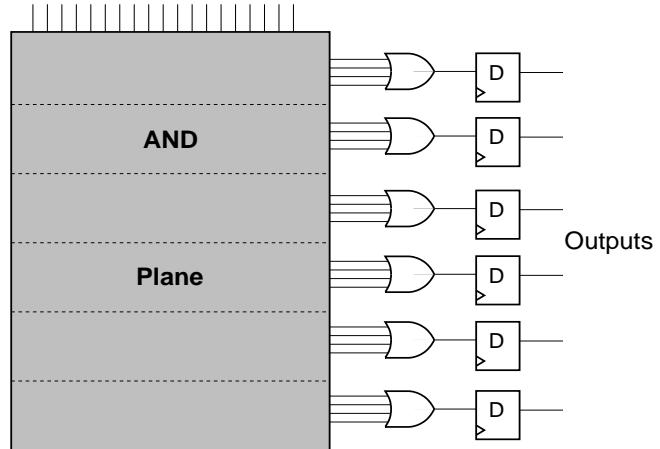
\includegraphics[width=\textwidth, height=0.6\textheight, keepaspectratio]{img1/PAL.jpeg}\\
PAL(可编程阵列逻辑)结构示意图
\end{center}
\end{columns}
\end{frame}

\begin{frame}{简单可编程逻辑器件(SPLDs)}
\begin{itemize}
\tightlist
\item
    包括 PLA、PAL 和类似 PAL 的器件。
\item
    主要特点:

    \begin{itemize}
    \tightlist
    \item
    低成本。
    \item
    极高的引脚到引脚速度性能。
    \end{itemize}
\end{itemize}
\end{frame}

\begin{frame}{复杂可编程逻辑器件(CPLDs)}
\begin{itemize}
\tightlist
\item
    随着技术进步,SPLD 的容量限制使得 CPLD 应运而生。
\item
    结构:

    \begin{itemize}
    \tightlist
    \item
    将多个 SPLD 集成到单个芯片上,并通过可编程互连将它们连接起来。
    \end{itemize}
\item
    发展:

    \begin{itemize}
    \tightlist
    \item
    由 Altera 首创,推出 Classic EPLDs、MAX 5000、MAX 7000 和 MAX 9000
    系列。
    \end{itemize}
\item
    逻辑容量:

    \begin{itemize}
    \tightlist
    \item
    相当于约 50 个典型 SPLD 器件,但难以扩展到更高密度。
    \end{itemize}
\end{itemize}
\end{frame}

\begin{frame}{可编程门阵列(FPGAs)}
\begin{columns}[T]
\column{0.6\textwidth}
\begin{enumerate}
\tightlist
\item
\textbf{Mask-Programmable Gate Arrays (MPGAs)}:
\begin{itemize}
\tightlist
\item
传统门阵列,由预制的晶体管阵列组成,通过定制金属互连实现用户逻辑电路。
\item
缺点:
\begin{itemize}
\tightlist
\item
定制化涉及高昂的设置成本和较长的制造时间。
\end{itemize}
\end{itemize}
\item
\textbf{Field-Programmable Gate Arrays (FPGAs)}:
\begin{itemize}
\tightlist
\item
类似于 MPGA,但配置由最终用户通过编程完成。
\item
结构:
\begin{itemize}
\tightlist
\item
由未指定的电路元件(称为逻辑块)和互连资源组成。
\end{itemize}
\item
优势:
\end{itemize}
\end{enumerate}

\column{0.4\textwidth}
\begin{center}
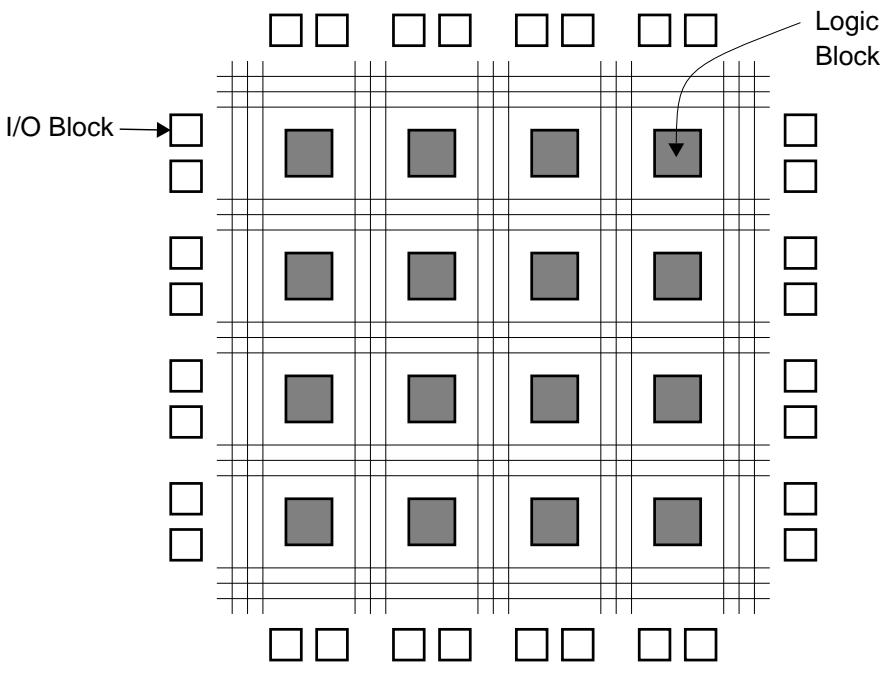
\includegraphics[width=\textwidth, height=0.6\textheight, keepaspectratio]{img1/FPGA.jpeg}\\
\textbf{图2:} \emph{FPGA结构图.}
\end{center}
\end{columns}
\end{frame}

\begin{frame}
\begin{block}{PLD 分类与逻辑容量}
\begin{itemize}
\tightlist
\item
    \textbf{SPLDs}:

    \begin{itemize}
    \tightlist
    \item
    容量最低,适合简单逻辑应用。
    \end{itemize}
\item
    \textbf{CPLDs}:

    \begin{itemize}
    \tightlist
    \item
    中等容量,适合中等复杂度设计。
    \end{itemize}
\item
    \textbf{FPGAs}:

    \begin{itemize}
    \tightlist
    \item
    最高容量,适合复杂逻辑设计。
    \end{itemize}
\item
    选择依据:

    \begin{itemize}
    \tightlist
    \item
    根据应用所需的逻辑容量。
    \end{itemize}
\end{itemize}
\end{block}
\end{frame}